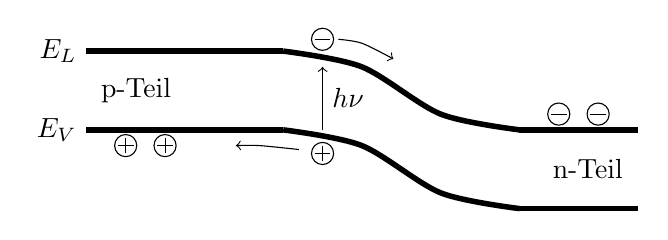
\begin{tikzpicture}
%Bänder
  \draw[line width=2pt] (0,2) -- (2.5,2);
  \draw[line width=2pt] plot [smooth] coordinates {(2.5,2) (3.5,1.8) (4.5,1.2) (5.5,1)};
  \draw[line width=2pt] (5.5,1) -- (7,1);
  \draw (0,2) node 
    [anchor=east]
    {$E_L$};
  \draw[line width=2pt] (0,1) -- (2.5,1);
  \draw[line width=2pt] plot [smooth] coordinates {(2.5,1) (3.5,0.8) (4.5,0.2) (5.5,0)};
  \draw[line width=2pt] (5.5,0) -- (7,0);
  \draw (0,1) node 
    [anchor=east]
    {$E_V$};
%Beschriftung
  \draw (1.2,1.5) node
    [anchor=east]
    {p-Teil};
  \draw (5.8,0.5) node
    [anchor=west]
    {n-Teil};
%Teilchen
  \draw (3,2.15) circle (4pt);
  \draw (2.9,2.15) -- (3.1,2.15);
  \draw (6,1.2) circle (4pt);
  \draw (5.9,1.2) -- (6.1,1.2);
  \draw (6.5,1.2) circle (4pt);
  \draw (6.4,1.2) -- (6.6,1.2);
  \draw[->] plot [smooth] coordinates {(3.2,2.15) (3.5,2.1) (3.9,1.9)};

  \draw (3,0.7) circle (4pt);
  \draw (2.9,0.7) -- (3.1,0.7);
  \draw (3,0.6) -- (3,0.8);
  \draw (1,0.8) circle (4pt);
  \draw (0.9,0.8) -- (1.1,0.8);
  \draw (1,0.7) -- (1,0.9);
  \draw (0.5,0.8) circle (4pt);
  \draw (0.4,0.8) -- (0.6,0.8);
  \draw (0.5,0.7) -- (0.5,0.9);
  \draw[->] plot [smooth] coordinates {(2.7,0.75) (2.2,0.8) (1.9,0.8)};

  \draw[->] (3,1.0) -- (3,1.8);
  \draw (3,1.4) node
    [anchor=west]
    {$h\nu$};
\end{tikzpicture}

